\documentclass{article}   

\usepackage{amssymb}
\usepackage{amsfonts}
\usepackage{hyperref}
\usepackage{eqnarray,amsmath}
\usepackage[table]{xcolor}
%
% \usepackage{mathptmx}      % use Times fonts if available on your TeX system
%
% insert here the call for the packages your document requires
%\usepackage{latexsym}
% etc.
%
\usepackage{graphicx}
\usepackage[round]{natbib}

\usepackage[table]{xcolor}
\usepackage{rotating}
\usepackage{caption}

%% if you use PostScript figures in your article
%% use the graphics package for simple commands
\usepackage{graphics}
\usepackage{natbib}


%% or use the graphicx package for more complicated commands
\usepackage{graphicx}
\usepackage[table]{xcolor}
% please place your own definitions here and don't use \def but
% \newcommand{}{}
%
% Insert the name of "your journal" with
% \journalname{myjournal}
%
\begin{document}

\title{Exercises of chapter 2}


\maketitle
Mayra Cristina Berrones Reyes

\section{Complexity experiments}

To compare the complexity of the best case, worst case, and average case, several sorting algorithms can be executed, giving it as an input, one at the time, all possible permutations of an array. \\

Performing multiple replicas with each entry to establish a typical execution time (to counteract the noise introduced by the operating system with its scheduling algorithms and other activities that take place on the computer) the permutation with the shortest execution time is the best case , the longest time is the worst case and the average among all these permutations is the average case in experimental terms. By increasing the number of elements in the array, it is possible to estimate the shape of the asymptotic growth curves of better and worse case as well as the average case. Some algorithms win in one aspect while losing in another. Which algorithm is good in what circumstances? In general, no reasonable algorithm will always be better to all the others.\\


\section{Sorting algorithms}

A sorting algorithm is made up from a series of instructions that take a list of elements, performs several operations (depending on the algorithm) and has as an output the list but sorted. To select the best suited algorithm for our array, we must compare their performance to see which one is best. The two performance metrics for this type of algorithms are time and space complexity. \\

In this experiments we will see the behavior of different sorting algorithms through their time complexity.\\

\subsection{Time complexity}

Big O notation is useful when analyzing algorithms for efficiency. For example, the time (or the number of steps) it takes to complete a problem of size n. The algorithms we are going to be experimenting with are the ones shown in Table \ref{ta1}.

\begin{table}[h!]
\centering
 \caption{Time complexity of the selected sorting algorithms} 
 \label{ta1}
 \begin{tabular} {| l | c | c | c |}
 \hline
Algorithm	&	$	Best-case	$	&	$	Worst-case	$	&	$	Average-case	$	\\
\hline
Bubble sort	&	$	O(n)	$	&	$	O(n^2)	$	&	$	O(n^2)	$	\\
\hline
Selection sort	&	$	O(n^2)	$	&	$	O(n^2)	$	&	$	O(n^2)	$	\\
\hline
Insertion sort	&	$	O(n)	$	&	$	O(n^2)	$	&	$	O(n^2)	$	\\
\hline
Heap sort	&	$	O(n log(n))	$	&	$	O(n log(n))	$	&	$	O(n log(n))	$	\\
\hline
Merge sort	&	$	O(n log(n))	$	&	$	O(n log(n))	$	&	$	O(n log(n))	$	\\
\hline
Quick sort	&	$	O(n log(n))	$	&	$	O(n^2)	$	&	$	O(n log(n))	$	\\
\hline
 \end{tabular}
 \end{table}
 
The idea of this experiment is to measure the time it takes each of this sorting algorithms to sort all the permutations of arrays of different sizes. The permutation with the least amount of processing time will be the best case scenario, the permutation with the bigest processing time will be the worst case scenario, and the average of all of the processing times will be the average case. \\

In this experiment we use several libraries on python to help us build this arrays faster, such as \textit{random} to build an array with different numbers each iteration, and \textit{itertools} to calculate all the permutations of the array. In Figure \ref{librerias} we see the two functions to create an array, and a list with all its permutations.\\

 

\begin{figure}[htp]
	\centering
	\caption{Excerpt of the code used in this experiment}
	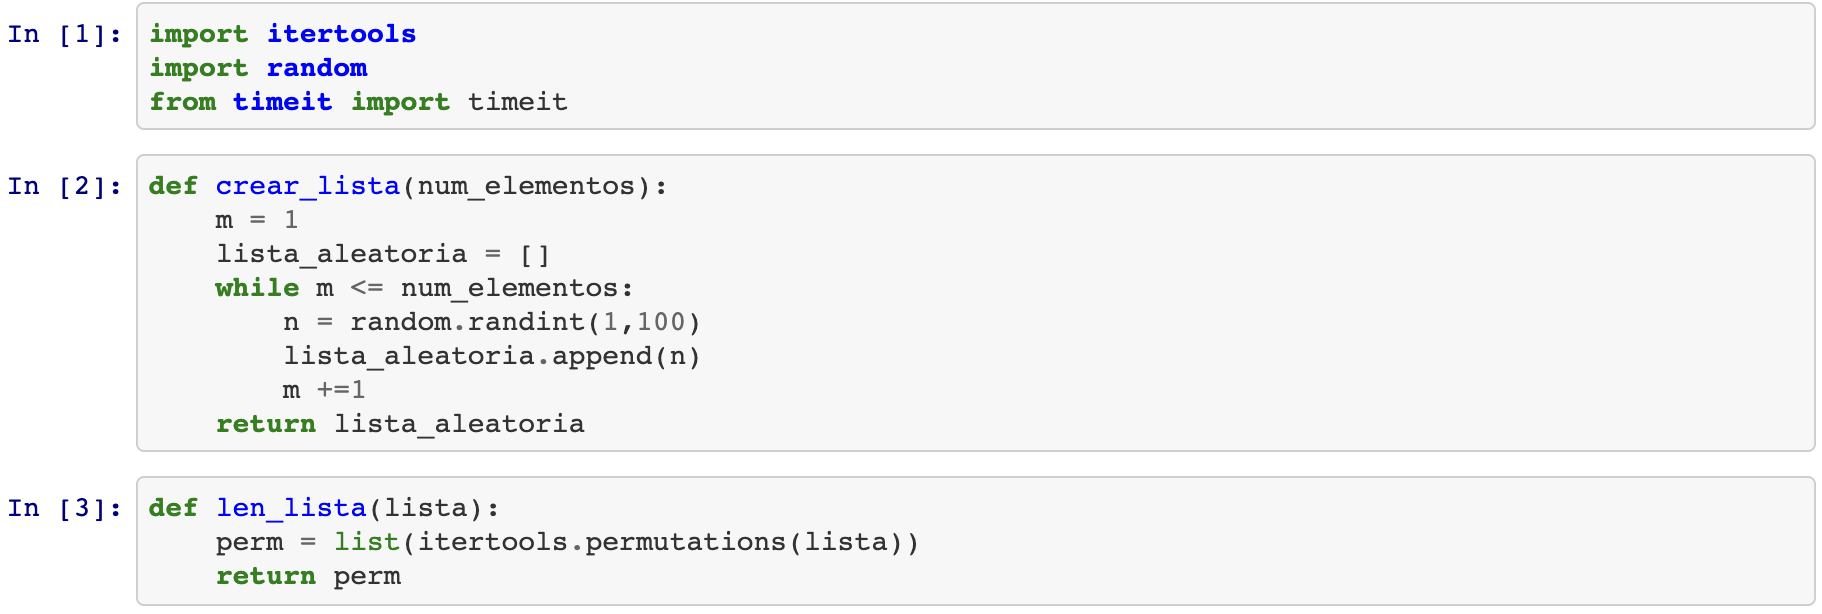
\includegraphics[width=\linewidth]{librerias.png}
	\label{librerias}

\end{figure}

In every number of elements, we made 100 iterations of arrays with different elements in it. We began with 4 elements, and kept adding one until we reached 9 elements. To see how many permutations had each array, we only needed to know the factorial of the number of elements. This is exemplified in Table \ref{ta2}.


 \begin{table}[h!]
\centering
 \caption{Number of permutations for each number of elements on the arrays.} 
 \label{ta2}
 \begin{tabular} {| r | r | }
 \hline
Number of elements&	Factorial of number\\
\hline
4 & 24 \\
\hline
5 & 120\\
\hline
6 & 720 \\
\hline
7 & 5040\\
\hline
8 & 40320\\
\hline
9 & 362880\\
\hline
 \end{tabular}
 \end{table}
 
 
 From Table \ref{ta3} to \ref{ta8} we calculated the average of all 100 iterations of the best and worst cases, as well as an average of the average cases in all 6 sorting algorithms. Later, form Figures \ref{ima1} to \ref{ima6} we show the best, worst, and average cases in a graphic of each of the algorithms.\\
 
   \begin{table}[h!]
\centering
 \caption{Description of the average of the 100 iterations in the best, worst and average cases of the \textbf{bubble sort algorithm}. } 
 \label{ta3}
 \begin{tabular} {| c | r | r | r | }
 \hline
Number of 	&		&		&		\\
 elements	&		$	Best-case	$	&	$	Worst-case	$	&	$	Average -case	$	\\
 \hline
4	&	$	2.0425x10^{-05}	$	&	$	2.1887x10^{-06}	$	&	$	5.3192x10^{-06}	$	\\
 \hline
5	&	$	1.6544x10^{-05}	$	&	$	2.1362x10^{-06}	$	&	$	5.4265x10^{-06}	$	\\
 \hline
6	&	$	3.8385x10^{-05}	$	&	$	1.7094x10^{-06}	$	&	$	5.7338x10^{-06}	$	\\
 \hline
7	&	$	9.4707x10^{-05}	$	&	$	2.0742x10^{-06}	$	&	$	7.1020x10^{-06}	$	\\
 \hline
8	&	$	1.7677x10^{-04}	$	&	$	2.2077x10^{-06}	$	&	$	8.7505x10^{-06}	$	\\
 \hline
9	&	$	1.2330x10^{-03}	$	&	$	2.1433x10^{-06}	$	&	$	1.0658x10^{-05}	$	\\
\hline
 \end{tabular}
 \end{table}
 
 
\begin{figure}[htp]
	\centering
	\caption{Graphic description of the behavior of the data colected in this experiment for the bubble sort algorithm}
	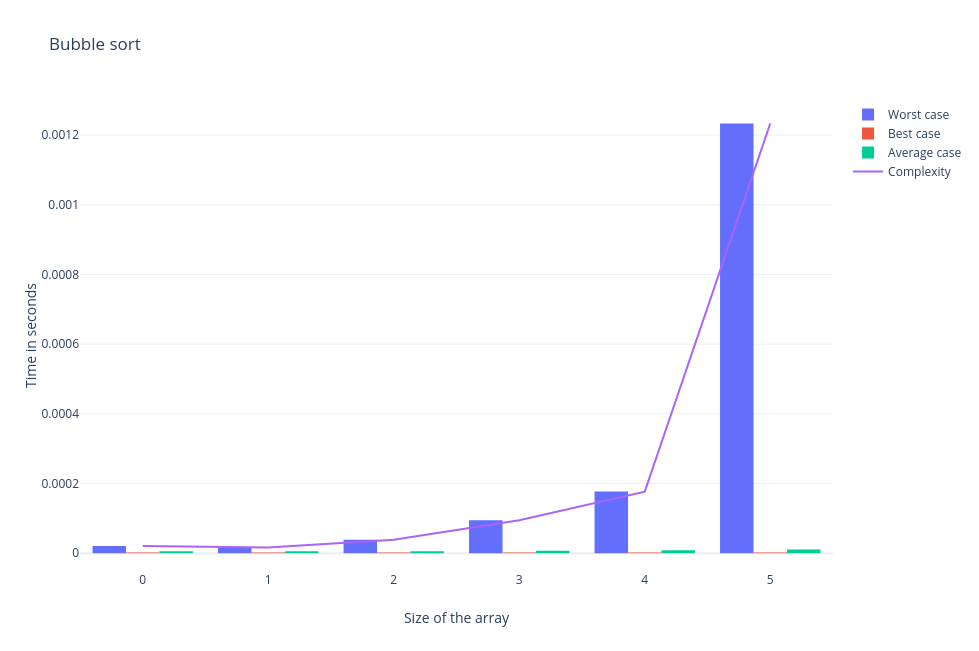
\includegraphics[width=\linewidth]{Bubblesort.png}
	\label{ima1}
\end{figure}

    \begin{table}[h!]
\centering
 \caption{Description of the average of the 100 iterations in the best, worst and average cases of the \textbf{selection sort algorithm}. } 
 \label{ta4}
 \begin{tabular} {| c | r | r | r | }
 \hline
Number of 	&		&		&		\\
 elements	&		$	Best-case	$	&	$	Worst-case	$	&	$	Average -case	$	\\
 \hline

4	&	$	4.9520x10^{-06}	$	&	$	3.3545x10^{-06}	$	&	$	4.0137x10^{-06}	$	\\
 \hline
5	&	$	2.0688x10^{-05}	$	&	$	4.0483x10^{-06}	$	&	$	5.0757x10^{-06}	$	\\
 \hline
6	&	$	8.5609x10^{-05}	$	&	$	4.8876x10^{-06}	$	&	$	5.8708x10^{-06}	$	\\
 \hline
7	&	$	4.1342x10^{-04}	$	&	$	5.5790x10^{-06}	$	&	$	6.8088x10^{-06}	$	\\
 \hline
8	&	$	1.2736x10^{-03}	$	&	$	6.3324x10^{-06}	$	&	$	7.4544x10^{-06}	$	\\
 \hline
9	&	$	3.8825x10^{-03}	$	&	$	7.1430x10^{-06}	$	&	$	8.7374x10^{-06}	$	\\
\hline
 \end{tabular}
 \end{table}

\begin{figure}[htp]
	\centering
		\caption{Graphic description of the behavior of the data colected in this experiment for the selection sort algorithm}
	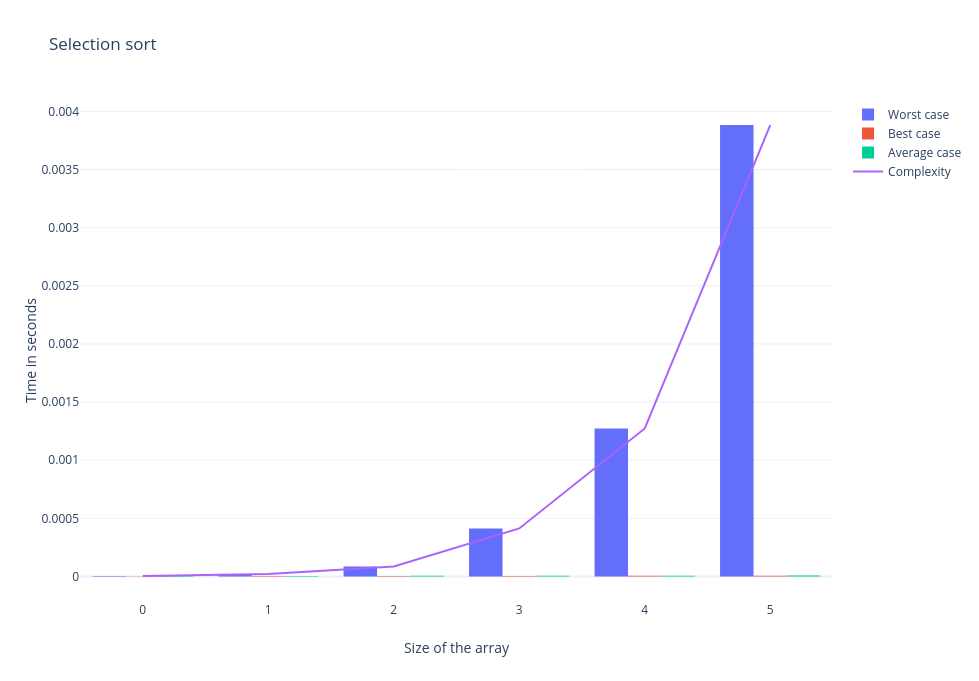
\includegraphics[width=\linewidth]{Selectionsort.png}
	\label{ima2}
\end{figure}

    \begin{table}[h!]
\centering
 \caption{Description of the average of the 100 iterations in the best, worst and average cases of the \textbf{insertion sort algorithm}. } 
 \label{ta5}
 \begin{tabular} {| c | r | r | r | }
 \hline
Number of 	&		&		&		\\
 elements	&		$	Best-case	$	&	$	Worst-case	$	&	$	Average -case	$	\\
 \hline
4	&	$	3.9959x10^{-06}	$	&	$	1.6856x10^{-06}	$	&	$	2.5314x10^{-06}	$	\\
\hline
5	&	$	3.1478x10^{-05}	$	&	$	2.5105x10^{-06}	$	&	$	4.2121x10^{-06}	$	\\
\hline
6	&	$	5.6040x10^{-05}	$	&	$	2.3532x10^{-06}	$	&	$	3.6283x10^{-06}	$	\\
\hline
7	&	$	5.1801x10^{-04}	$	&	$	2.3937x10^{-06}	$	&	$	4.3553x10^{-06}	$	\\
\hline
8	&	$	1.1991x10^{-03}	$	&	$	2.7704x10^{-06}	$	&	$	4.9595x10^{-06}	$	\\
\hline
9	&	$	2.5292x10^{-03}	$	&	$	3.0589x10^{-06}	$	&	$	5.6250x10^{-06}	$	\\
\hline
 \end{tabular}
 \end{table}

\begin{figure}[htp]
	\centering
		\caption{Graphic description of the behavior of the data colected in this experiment for the insertion sort algorithm}
	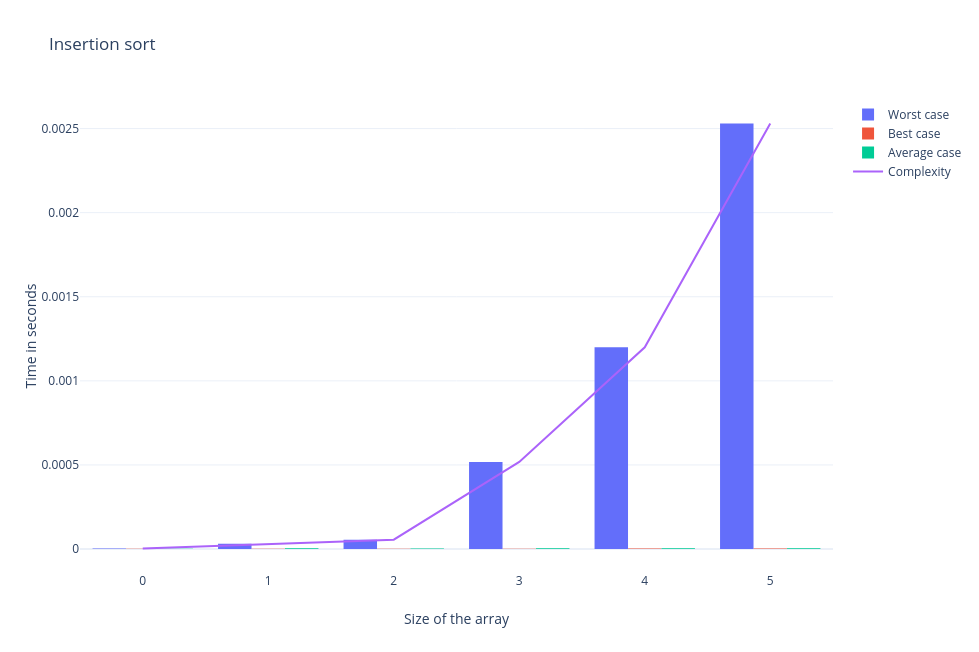
\includegraphics[width=\linewidth]{Insertionsort.png}
	\label{ima3}
\end{figure}

     \begin{table}[h!]
\centering
 \caption{Description of the average of the 100 iterations in the best, worst and average cases of the \textbf{heap sort algorithm}. } 
 \label{ta6}
 \begin{tabular} {| c | r | r | r | }
 \hline

Number of 	&		&		&		\\
 elements	&		$	Best-case	$	&	$	Worst-case	$	&	$	Average -case	$	\\
 \hline
4	&	$	1.2109x10^{-05}	$	&	$	5.5647x10^{-06}	$	&	$	7.0568x10^{-06}	$	\\
 \hline
5	&	$	8.3866x10^{-05}	$	&	$	6.4063x10^{-06}	$	&	$	9.0000x10^{-06}	$	\\
 \hline
6	&	$	1.4008x10^{-04}	$	&	$	7.7701x10^{-06}	$	&	$	1.0264x10^{-05}	$	\\
 \hline
7	&	$	6.2078x10^{-04}	$	&	$	8.9073x10^{-06}	$	&	$	1.2097x10^{-05}	$	\\
 \hline
8	&	$	1.9230x10^{-03}	$	&	$	1.0705x10^{-05}	$	&	$	1.4125x10^{-05}	$	\\
 \hline
9	&	$	6.5225x10^{-03}	$	&	$	1.2009x10^{-05}	$	&	$	1.6323x10^{-05}	$	\\
\hline
 \end{tabular}
 \end{table}


\begin{figure}[htp]
	\centering
		\caption{Graphic description of the behavior of the data colected in this experiment for the heap sort algorithm}
	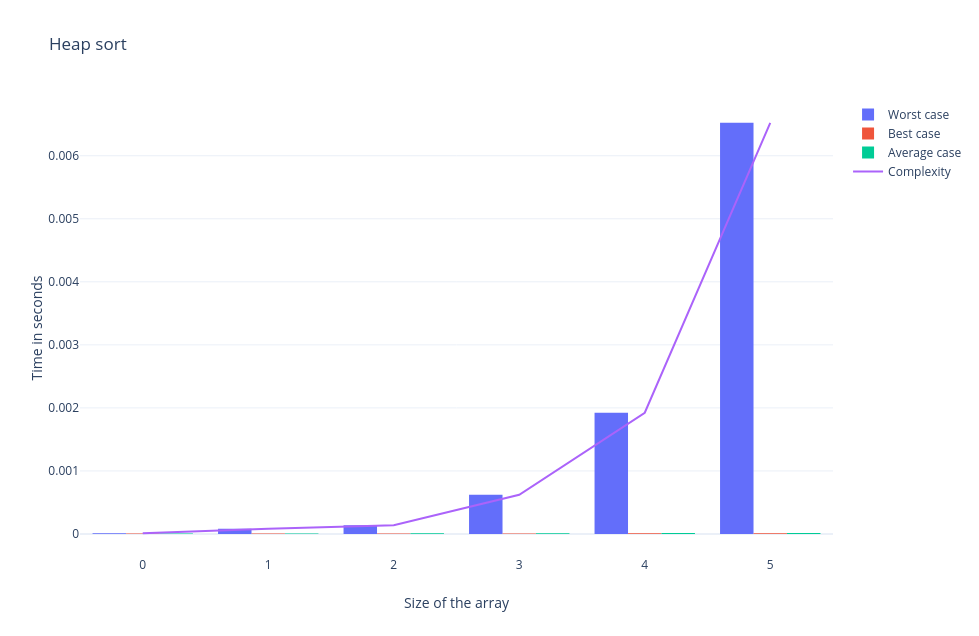
\includegraphics[width=\linewidth]{Heapsort.png}
	\label{ima4}
\end{figure}

     \begin{table}[h!]
\centering
 \caption{Description of the average of the 100 iterations in the best, worst and average cases of the \textbf{merge sort algorithm}. } 
 \label{ta7}
 \begin{tabular} {| c | r | r | r | }
 \hline

Number of 	&		&		&		\\
 elements	&		$	Best-case	$	&	$	Worst-case	$	&	$	Average -case	$	\\
 \hline

4	&	$	1.1375x10^{-05}	$	&	$	6.2943x10^{-06}	$	&	$	7.5241x10^{-06}	$	\\
 \hline
5	&	$	3.9556x10^{-05}	$	&	$	8.0180x10^{-06}	$	&	$	9.1617x10^{-06}	$	\\
 \hline
6	&	$	1.3530x10^{-04}	$	&	$	9.9039x10^{-06}	$	&	$	1.1302x10^{-05}	$	\\
 \hline
7	&	$	8.1806x10^{-04}	$	&	$	1.1654x10^{-05}	$	&	$	1.3662x10^{-05}	$	\\
 \hline
8	&	$	1.6717x10^{-03}	$	&	$	1.3838x10^{-05}	$	&	$	1.5335x10^{-05}	$	\\
 \hline
9	&	$	1.5808x10^{-03}	$	&	$	1.6322x10^{-05}	$	&	$	1.8028x10^{-05}	$	\\
\hline
 \end{tabular}
 \end{table}

\begin{figure}[htp]
	\centering
		\caption{Graphic description of the behavior of the data colected in this experiment for the merge sort algorithm}
	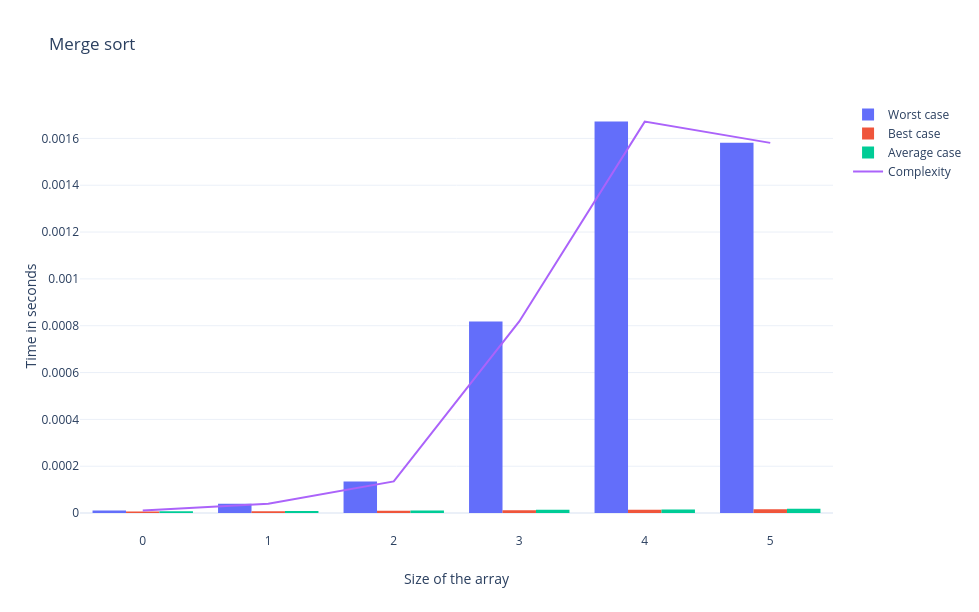
\includegraphics[width=\linewidth]{Mergesort.png}
	\label{ima5}
\end{figure}

     \begin{table}[h!]
\centering
 \caption{Description of the average of the 100 iterations in the best, worst and average cases of the \textbf{quick sort algorithm}. } 
 \label{ta8}
 \begin{tabular} {| c | r | r | r | }
 \hline

Number of 	&		&		&		\\
 elements	&		$	Best-case	$	&	$	Worst-case	$	&	$	Average -case	$	\\
 \hline

4	&	$	2.5382x10^{-05}	$	&	$	3.8815x10^{-06}	$	&	$	5.7858x10^{-06}	$	\\
 \hline
5	&	$	6.3350x10^{-05}	$	&	$	4.9305x10^{-06}	$	&	$	6.6607x10^{-06}	$	\\
 \hline
6	&	$	1.9596x10^{-04}	$	&	$	5.4264x10^{-06}	$	&	$	7.4335x10^{-06}	$	\\
 \hline
7	&	$	3.9595x10^{-04}	$	&	$	6.5613x10^{-06}	$	&	$	8.2383x10^{-06}	$	\\
 \hline
8	&	$	1.5688x10^{-03}	$	&	$	7.2289x10^{-06}	$	&	$	9.1766x10^{-06}	$	\\
 \hline
9	&	$	1.5300x10^{-03}	$	&	$	8.5521x10^{-06}	$	&	$	1.0223x10^{-05}	$	\\
\hline
 \end{tabular}
 \end{table}
 
 
\begin{figure}[htp]
	\centering
		\caption{Graphic description of the behavior of the data colected in this experiment for the quick sort algorithm}
	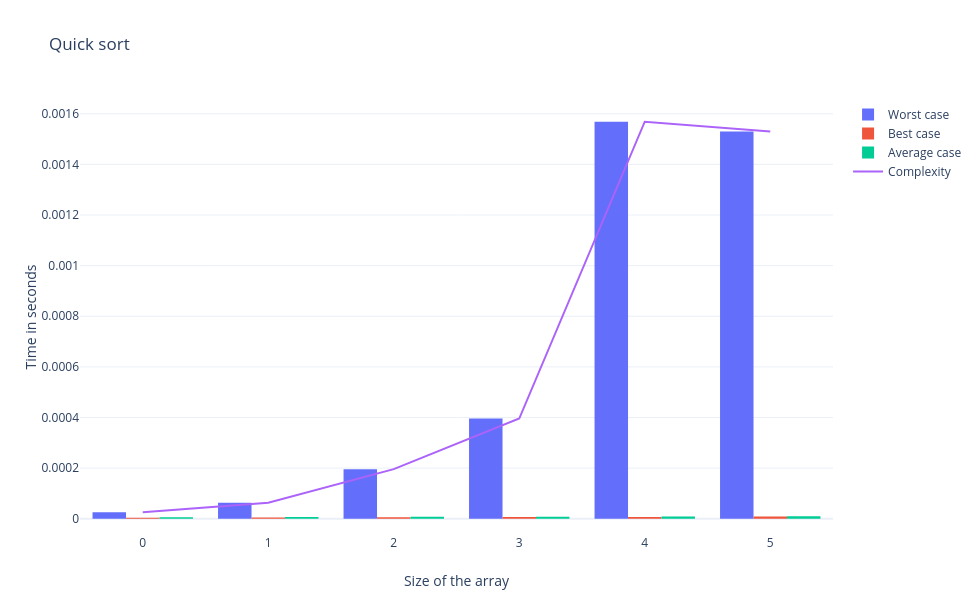
\includegraphics[width=\linewidth]{Quicksort.png}
	\label{ima6}
\end{figure}

Lastly we have the Figures \ref{ima7}, \ref{ima8}, \ref{ima9} in which we put all the sorting algorithms together and showed them divided by best, worst, and average to see better the contrast between all the algorithms performances.\\
\begin{figure}[htp]
	\centering
		\caption{Graphic description of the average of the best cases of all of the sorting algorithms used in this experiments}
	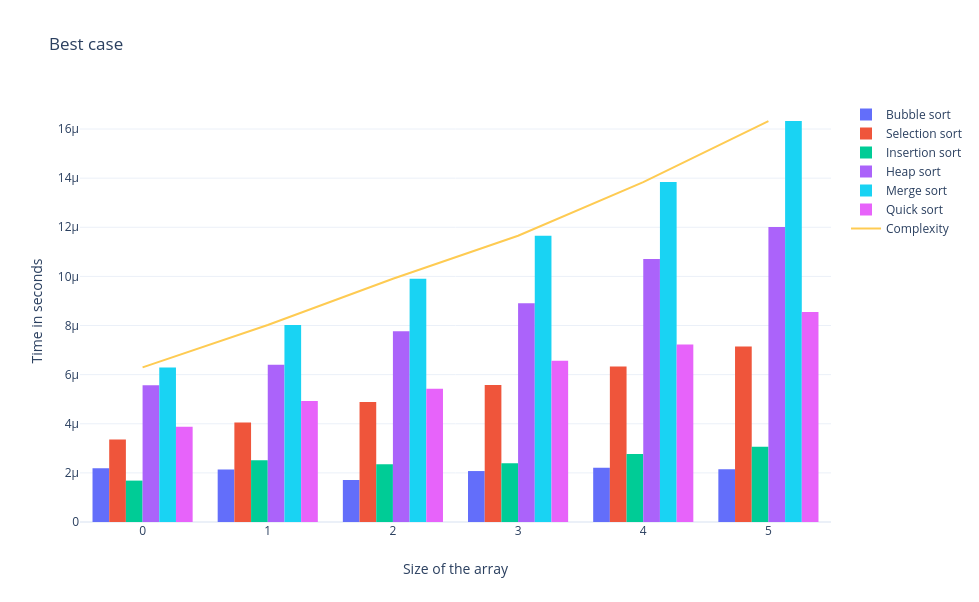
\includegraphics[width=\linewidth]{Bestcase.png}
	\label{ima7}
\end{figure}

\begin{figure}[htp]
	\centering
	\caption{Graphic description of the worst of the best cases of all of the sorting algorithms used in this experiments}
	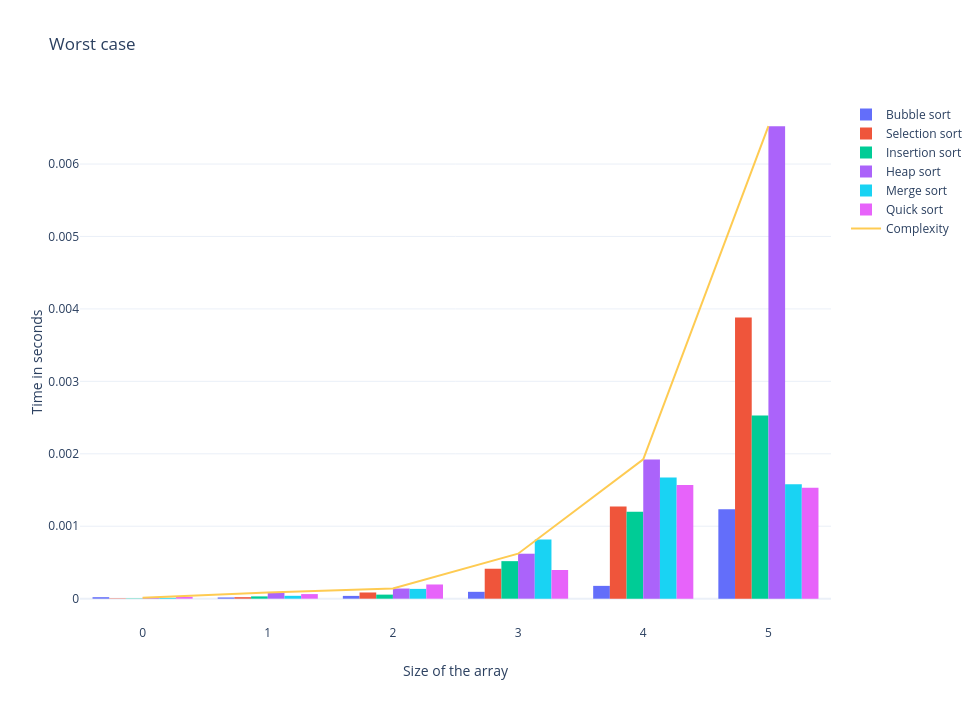
\includegraphics[width=\linewidth]{Worstcase.png}
	\label{ima8}
\end{figure}

\begin{figure}[htp]
	\centering
	\caption{Graphic description of the average of the average cases of all of the sorting algorithms used in this experiments}
	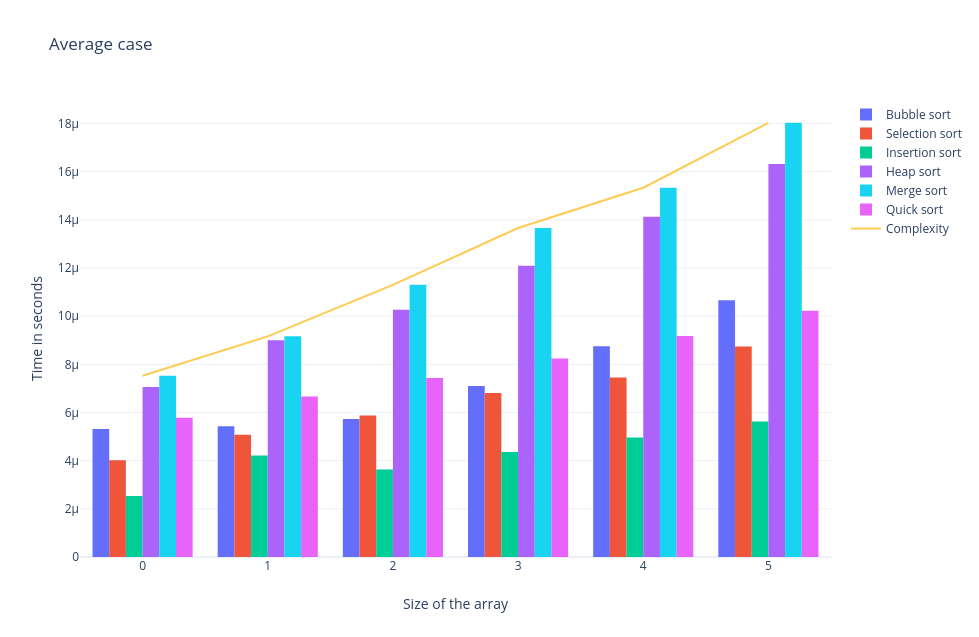
\includegraphics[width=\linewidth]{Averagecase.png}
	\label{ima9}
\end{figure}

 \section{Conclusions} 
 
After reading some things about the complexity of time in this algorithms, and the concept of big O, reviewing the results of the tables and figures, they seem to fit in the normal behavior for each type of algorithm. \\

Reading further into the results, we see that all of the algorithms seem to have a similar performance in the size 4, 5, and 6 of elements on the array, and it is very clear in Figure \ref{ima8} that the bigger the number of elements in the array, the complexity increases.\\

There is a slight change in the Figure \ref{ima4} in the end, where the complexity lowers. This can be attributed to heap sort algorithms are not stables, same as the quick sort algorithm. This is one of the reasons we need to know the complexity in the best, worse, and average case, so we can decide if its worth to spend it all on a stable but slow algorithm, or if it might be worth the trouble of implementing an algorithm that is not as stable, but has a better performance on average for bigger amount of elements in the array.\\

 
\end{document}